\chapter{草稿之一——当代艺术——版本0.2}

\section{当代艺术的概念}

什么是当代艺术,它具体起源于何时,主要表现是什么?像艺术的概念一样,并没有一个确
定而公认的答案。在众说纷纭的“当代艺术”概念阐述中,往往也存在着观念艺术、后现代
艺术、当代艺术这三者之间界限不明、混淆不清或者顾此失彼的问题。

在《詹森艺术史》中,只介绍了比较细分的观念艺术和后现代艺术等,没有单独提及当代艺
术 。但笔者认为,但《詹森艺术史》后现代时代一章中关于艺术哲学理论发展和影响的阐释
较为精准到位和克制。

\begin{quotation}
  20世纪80年代以来,艺术界关注的艺术风格通常被称为后现代艺术(Postmodern
  art)。60年代中期,欧洲文学评论界确定了“后现代”这一术语的含义,并首先在文学领
  域使用;这个圈子的核心人物是法国哲学家雅克·德里达(Jacques
  Derrida,1930-2004年),其理论也被称为“解构主义”(Deconstructionism)或“后结
  构主义”(Post-Structuralism)。\medskip

  50年代和60年代期间,罗伯特·劳申伯格、安迪·沃霍尔和罗伊·利希滕斯坦都对这一问题很
  感兴趣。虽然后现代主义在视觉艺术领域的灵感来源就是这个时期,但艺术界真正自觉进
  入新时代的情况直至70年代晚期才出现。\pagescite[][1077]{9787510048623}\medskip

  他们还受到另一位法国后现代哲学家或后解构主义哲学家让·鲍德里亚(Jean
  Baudrillard,1929-2007年)的影响,后者的拟像(simulacrum)理论影响尤为重
  大。……超级现实,通过包含电影、电视在内的大众媒体,美国人创造了一个虚假、完美、
  永恒的世界,仿佛比现实本身更加“真实”……\pagescite[][1094]{9787510048623}
\end{quotation}

国内王端廷在《西方现代、后现代和当代艺术的分期与区别》一文中,将后现代艺术风格断
代为1979-1989年,当代艺术风格断代为1989年至今。并提出“对审美的回归是当代艺术的
总趋势”,“什么都是艺术”,“人人都是艺术家”的观点已经过时。但是我们看到,王瑞
廷文中所说当代艺术的“普世主义”仍未脱出后现代理论语境,仍是用后现代理论作为指导。
\cite{wangduanting}

周计武在《什么是当代艺术》一文中,认同阿瑟·丹托和汉斯·贝尔廷的看法,过往被叙事逻
辑支配的时期被称为“艺术的时代”,即艺术在其中具有明确的历史方向和历史意义的时代。
它开端于文艺复兴时期,终结于20世纪60年代,被如今没有大师叙事的后历史时代所取代。
在丹托看来,“后现代”一词过于暖昧,既可指现代之后的艺术,也可指现代艺术体系内的自
我批判。因此,丹托主张用“当代艺术”替代“后现代艺术”一词。\cite{whatsart}但令人
奇怪的是,周计武为何将79年的“星星”美展和“85美术新潮”定为当代艺术,看其表达形
式和内容、意义,笔者认为,这应当还是算作现代艺术。

笔者认为,周计武所提到的内容是当代中国最为广泛接受的“当代艺术”概念——来源于丹托
“艺术终结”论的观点。
\begin{quotation}
  “艺术死亡”、“艺术史结束”、“人人都是艺术家” 的呼声,在当代欧美美学界和艺术
界越来越高 ,对中国本土的美学和艺术也开始产生重要影响。这些 “空洞口号” 既非艺术
家也非纯美学家所创,而是肇始于当代美国分析哲学家阿瑟·丹托 (Arthur C.Danto)的 “艺
术终结” (the End of Art) 的宣称。\cite{boduoyishu}
\end{quotation}

如贡布里希所说,对艺术风格整齐的年代划分只是艺术史家或艺术史爱好者所喜欢用的方法,
不可能有一个绝对正确时间段的当代艺术划分,但上述所提及的当代艺术概念其实是求同存
异的,尤其是在后现代理论对他们的影响方面。

结合实际,在当前国内当代艺术作品鉴赏中,抽象的、底层的理论方面,我们看到策展人、
艺术家自称的铺天盖地的“解构”、“拆解”、“碎片化”以及德里达、利奥塔、福柯、鲍德里
亚等人的后结构、后现代理论引用和更早提出“反艺术”的阿多尔诺的理论。

在通俗具体的当代艺术解释上,国人则喜欢用“反艺术”,“人人都是艺术家”,“不止审
美也审丑”,“重要的是理念,而非形式”“一切皆可”等丹托的“艺术终结论”观点。其
实就丹托文章内容和参考文献来看,丹托“艺术终结论”的提出应该也是受德里达曾前提出
的文学、历史等终结论的影响。

本文将从丹托“艺术终结论”和后现代理论两个方面来考察当代艺术。

\section{后现代理论起源和发展}
\unsure[inline]{这一节先留着,对理论不感兴趣的人可以不看。不排除以后将当代艺术一
  节归入后现代章节下,届时本节将归入后现代。}

对于后现代理论从何时开始发展,没有一个唯一的答案。较多人接受后现代发起于20世纪中
后期,道格拉斯·凯尔纳和斯蒂文·贝斯特认为真正提出一个新的后现代纪元这一观点的是法
国的鲍德里亚和利奥塔。法国最先宣扬历史出现后现代断裂受几个方面影响:法国二战后出
现的迅猛的现代化进程,农业为基础的社会变成了主要以城市和工业为基础的社会,资本主
义带来高速发展的生产力和科学技术;五六十年代哲学和社会理论所取得的令人振奋的进步,
马克思主义、存在主义、现象学被语言学倾向的结构主义和拉康精神分析所代替;1968年法
国五月风暴所引发的强烈的决裂感,许多人开始反思马克思主义,尤其是法共所讲的马克思
主义是否过于教条和狭隘甚至是压迫性的,不能从理论上说明当代社会及其多样化的权利样
式,并且批判了把知识当成获取权力和统治工具的做法,也批判了自由主义制度在解决民众
不满情绪方面的无能。

结构主义进一步发展为后结构主义(解构主义)。后结构主义把能指\footnote{语言符号中
  的视听acoustic visual成份,今天被解释为可被听、闻、触、视、尝到的物质形式}放在比所
指\footnote{语言符号中的概念性成分}更重要的位置上,以此来表明语言的动态生产性和意
义的不稳定性,表明他们同意义的再现图式的决裂。他们认为能指仅仅是无休止的指意
(signification)过程中的一个瞬间。在这个过程中,意义仅仅是在所指的无限的、模棱两
可的游戏中生成的。代表人物德里达则成为后来一些后现代文学、艺术风格的理论建基者。

后结构主义逐步迈向多种多样的后现代理论。本文的主旨不在于具体阐述这些理论,而是在
于当代艺术批判,在此略过不表。

有意思的是,福柯、鲍德里亚均参加过法国共产党,并于50年代初退出。德里达则可以算是
个修正的后马克思主义者,而利奥塔也曾是马克思主义者,后来成为了背弃的后马克思主义
者。

\section{丹托的艺术终结论}

\subsection{丹托艺术终结论概览}丹托的“艺术终结”并不是字面意思上的不再有艺术
了,丹托想表达的是以往叙事的艺术史已经终结,被如今没有大师叙事的后历史时代所取代。
“一个没有历史方向、历史意义和叙事导向的艺术”。

丹托认为,“艺术哲学史就是哲学压抑、剥夺艺术的历史。这与尼采的观点不谋而
合。”\cite{dantuozhenduan}这一哲学压抑艺术的历史向前可追溯至柏拉图的艺术模仿论,
在近代20世纪来看的话,则是:

\begin{quotation}

  请想想我们世纪令人眼花缭乱的一连串艺术,如野兽派、种种立体主义的表现、未来主义、
  漩涡主义、同步主义、抽象主义、达达派、表现主义、抽象表现主义、波普艺术、欧普(光
  效应)艺术、极简主义、后极简主义、观念主义、照相写实主义、新表现主义。(他们的寿
  命长则两三年,短则一个半月,且是“令人烦恼的艺术”。)……艺术的命令其实就是历史
  的命令——创造一个艺术史时期吧!——而成功就在于制造一种公认的新事物中。

  每个时期需要相当数量的相当复杂的理论,以便也能在艺术层面上处理时常是很微小的对
  象。面对历史定位与理论解放的深刻相互作用,对感情和表现的呼吁似乎越来越没说服力了。
  即使在今天,我们几乎也不明白立体主义几乎是怎么回事,但我确信在布拉克和毕加索宣布
  他们对吉他惊人一致的感情之后还有许多值得玩味的东西。
  \pagescite[][122]{7214029774}

  这些前不久的作品显示了另一种特色,那就是对象接近于零(前文提出的作品中在艺术层
  面上处理时常是很微小的对象),而其理论却接近于无限,因此一切实际上只是理论,艺
  术在对于自身纯粹思考的耀眼光芒中蒸发掉了,留存下来的,仿佛只是作为它自身理论意
  识对象的东西。\pagescite[][126]{7214029774}

  事实上,当艺术认识到一件艺术品不一定要成为某种特定的方式时,当艺术终结时,这种
  叙事就终结了。……追求哲学认同的艺术史结束了。艺术的价值就在于它允诺的自由:一种
  摆脱惨淡的人生境遇和冷酷的生活秩序的自由,一种自律的、审美的、不食人间烟火的“自
  由”。……在丹托看来,这种把美的艺术与生活分离开的“分类的权力就是统治的权力,而
  这些类似的审美状态(艺术哲学理论家的审美观)应被视为对双方感到的隐藏危险做出的反
  应,它本质上是政治性的。”\cite{dantuozhenduan}

\end{quotation}

丹托认为过往压抑或剥夺艺术权力的艺术哲学史模式被颠覆或“终结”,取而代之的是一种
新的“一切皆可、一切皆得为艺术”的“后历史”新艺术哲学。当代艺术来临了!

\subsection{丹托艺术终结论批判}

\begin{quotation}

如果一切皆可,那恰恰成了一切皆不可……没有真理的断言,就没有激情,一切皆可,彼此彼
此,就将导致相对主义、犬儒主义与虚无主义。但是丹托似乎高兴地宣告这一时代的来临,却
不认为这足一种危机的症状。\cite{fuwendantuo}

类似“一切都能成为艺术品”、“每个人都是艺术家”的口号,成为新的教条。这种深层结
构上的复数主义,一方面,满足了大众对意义的追求,颠覆了现代主义叙事的精英倾向;另
一方面,丧失了历史的意义和方向,暗合了新型中产阶级的意识形态要求。在某种程度上,
它终结了不断进步的艺术史叙事。\cite{dantuozhenduan}
\end{quotation}

丹托的理论中,似乎是将艺术置于一个相当超然的位置之上,艺术在这里与政治、经济、科
技、生活等彻底分割开来,单独提前步入了丹托所说的马克思的乌托邦社会——没有界限的,
绝对自由的后历史精神社会。这怎么可能呢?!这简直是一个哲学门外汉及现实门外汉的想
象!在时间上和话语上,丹托应当是从德里达那里看到并拓展了“终结”。但丹托的理论中
却完全没有后现代理论中对现代性的批判成分,号称继承了尼采的多元主义、反理论压迫、
重酒神精神的生命哲学,最终却又完全背离了尼采,成为空洞的,毫无生机和反抗精神的虚
无。笔者甚至认为,丹托完全不了解后现代理论,只是肤浅借用。

同时,丹托反艺术界中狭隘审美和理论的美好愿望非但没有实现,反而使艺术界的权力上升
至艺术历史中前所未有的高度,使艺术彻底抛离了大众并成为权力手中的玩物。如果说过往
的艺术霸权是通过关于审美和历史等方面的理论来实现的,如今的霸权则不需要任何理论就
可以实现。说你行你就行,说你不行就不行!

\section{结合后现代理论对当代艺术的批判}

当代艺术常有固定的范例和形式,这些范例和形式常被机械式地复制,创新为复制让路,崇
高为平庸让路,一切为艺术界让路,艺术界则为资本和权威让路。

% \begin{itemize}[noitemsep]      %
\begin{itemize}

\item 日常中随处可见的俗物,简单直露到可怕的类波普艺术展示。大圣啊,快收了神通吧。
朱熹和王阳明的“格物致知”,早在几百年前就吊打你们了。

\item 无人能懂的抽象,或者乱涂乱抹,层出不穷的棉花、各种材质的线和金属扭曲缠绕的
非具象,或者用当代艺术说法——当代艺术想赋予我们的,正是人人都可以有自己的理解。虽
然人人都是艺术家,而如果想对这种抽象进行“权威”解读并得到承认却需要依顺作者和权
威人士的语言文字。
  
\item 带血伤口、血盆大口、超大眼珠、流出或散落的人体器官……还有对生命伦理的蔑视,
劈成两半的动物,动物的头、器官和血。在80年代以前的纪实摄影师中,尤其是战地纪实摄
影师,都极少去直接拍摄惨烈战场上的死尸、伤口和鲜血,这被认为是以猎奇、刺激、低俗
的手法吸引观众,而将对战争和生命的反思置于二线。

\item 艳俗低俗的女性、男性裸体。人在此处往往只是充当物欲或者猎奇点。后现代理论中
的微观欲望政治就“欲望在其本质上是革命性的”进行了扩展讨论并寄予厚望,希望能借解
放自人类诞生之日起就有并伴随每人一生,促动人类社会发展变动的欲望、形成新的欲望方
式来突破现代性的辖域。但在当代艺术、后现代艺术中,肉体往往只是肉欲的、物化的或者
空洞的,这类艺术欲望毫无解放的张力,反被现代性彻底的役使所用。

\item 空洞乏味的行为艺术。阿布拉莫维奇2010年的《艺术家在现场》与男友乌雷的“偶然
相遇”是其最为人所知的艺术作品,常令富有文艺或憧憬爱情的男女们感动,笔者只想说,
来,干了这杯鸡汤!这鸡汤便是浓缩的艺术呵!噢,听说后来乌雷认为版权费给的太少,对
阿布拉莫维奇发起了诉讼,至于诉讼结果如何,笔者无意关注。
  
\item 直接空洞的房间,或黑或白或兼而有之,可加一两句话,再配上几盏闪亮的灯那自然
是最好不过。保守估计全世界有上千件这样形式的作品。“重要的是艺术家提出的观念,至
于形式是什么并不重要”。何苦去看这些不成形的东西呢?经典文史哲哪个不提出观念,哪
个不比你论述的更有感情、强度、深度……

\item 对中国国家政治、文化符号进行刻意的挑衅、抹黑,以此来获取一些西方不明真相群
众或反华势力的“关怀”,其中关于天安门的“当代艺术”是重灾区。出奇的是,这一点被
相当多的中国当代艺术家们前赴后继、乐此不疲地复制,还常能在国外各大小比赛中获奖。
就这点来说,中西方的当代艺术界同样是令人失望的,他们只是以所谓反中国霸权体制的名
头去投靠西方霸权体制而已。当代艺术的反政治是个天大的笑话。

\item 构成作品的单位元素数量众多,或作品面积、体积庞大,或超大场景,或耗费极大。

\item 被禁锢或污损的宗教文化符号,如笼中之佛,断头菩萨等。

\end{itemize}


丹托“艺术终结论”中,艺术界制度消失,但如本文上一节所说,艺术界的权力从未如此强
大过。当代艺术所标榜的表达观念往往要被如前所述的出位、猎奇、空洞的形式所遮蔽。如
果是还未出名的当代艺术家,除作品外还需要向“有关部门”递交artist statement(艺术
家自述);成名的艺术家在拿出作品后常要备上访谈录、演讲或者其他艺术家的理解说明;
艺术家们彼此写文、演讲,彼此歌功颂德,花花轿子人抬人、芝麻开花节节高,巩固加强自
己的权威;几个均小有名气的艺术家联合署名以扩大影响力;或在作品中向业内强力人士献
媚;在评比中评委们倾向于金钱或者权威或者派别;权威们不停地用让人摸不着头脑的堆积
在一起的无趣概念创造艺术的解读,或者自己生硬造出一种概念去巩固加强树立自己的权威,
在贪婪权威的作用下,他们看到了树立标准的巨大诱惑,他们已经可以像时尚界一样于今年
聚在一起定出明年流行的理论标准,并肯定会在会后某个时间找出几件适合“标准”的作品
大肆宣扬,使理论得到更好传播了,德里达、福柯、鲍德里亚,利奥塔的名字轮番循环上阵,
今年这句话,明年那句话……艺术圈的中低层们快速传播这些圈里权威创作的“今年流行
款”,圈外爱好者们则迷信权威,普通百姓对此毫不关心,这便是当代艺术里本应消失的艺
术界制度啊。

笔者对亲身经历的一事深感可怕。笔者参加展览极少,对策展人了解极少,但仅有的几次看
展常能见到某位客座教授、策展人为青年新锐、艺术家布展。这位教授的文案善于堆砌各种
专业术语和迷之感性,使笔者常常反胃恶心。荒诞的是笔者后来翻到一本很小众的访谈录,
访谈录里的这位策展人在书里深具远见卓识。也就是说,这位精神分裂的策展人在理论很足,
很懂人话的情况下,在策展时分裂为一个说鬼话的“大师”。笔者对此久久不能忘怀。

后现代理论在反对大师叙事、总体化、本质主义的道路上有时会走向相对立的另一个极端,
偶尔会产生与后现代理论始作俑者尼采的积极虚无所不同的消极虚无、并在总体和普遍上陷入
逻辑矛盾。但是后现代理论仍是有对现代性(很大程度上是资本主义的体现)的强烈批判,
并富有生机和张力。

而当代艺术只不过是挂着后现代的名头,后现代理论中的反规诫、反霸权、微观欲望、解辖
域化、重艺术的情感和强度只能是嘴皮说说而已。一切均被商品化、流水线化。因当代艺术
的本质虚无,资本更加轻易操纵和控制了艺术界。

鲍德里亚在《艺术的阴谋》里对当代艺术提出的批评比较直接尖锐:
\begin{quotation}
它们得到的是庸常性的成乘方的增长。它们自称自己无价值:“我是无价值的!我是无价
值的!”——而实际情况是,它们真的是无价值。

当代艺术全部的欺骗性就是:公开宣称自己无价值和无意义——当它已经是无价值的时候,声
称力争使自己无价值。当它们已经是无意义的时候,声称力争使自己无意义,并且声称要以
肤浅的语汇实现艺术的肤浅。\cite{artistyinmou}

艺术没有什么特殊的美学地位,没有特权——甚至负面的也没有。我的意思是,如果艺术在独
自承受规范失落、无价值的讽刺性的苦闷命运,这仍是一项特权和殊荣。然而一切事物——政
治、道德和哲学领域——都在向无价值的最小公约数进发。这不幸的同病相怜的命运本应是对
艺术的一种安慰,但其实它加强了艺术的无意义,艺术甚至不是独自处于无意义的境地——因
此事实上,它既无特殊的本质,也无特殊的位置。\cite{yishudexiaoshi}

\end{quotation}

中国的艺术批评还是太少,自艺术批评对印象派的斗争失败以来,艺术批评的生存空间越来
越窄,标榜反艺术的艺术界对于尖锐的批评也越来越不能容忍,当代艺术更是将批评驱逐至
蛮荒。仅有的批评,常过于片面偏激。如河清教授的美帝阴谋论,笔者认为,将美帝更改成
资本全球化(美国为首),将人的主观故意的阴谋改成资本的人格化或称资本强加给人的规
律似乎更能贴近客观;如试图扩展传统东方艺术文化比重,压制西方当代艺术空间的言论,
其实这种提法没有看到传统书画艺术虽然讲究技法,富有中国传统文化底蕴,有自己独特的
审美机制,但在被资本和权力辖制上,与当代艺术并未产生实质的区别。


\section{结语}

就我寥寥无几的看展经历,当前中国,富有社会关怀,人文关怀的作品并不多见。以艺术形
式来说,雕像、版画、油画、中国画是在社会关怀方面依次递减的,似乎与他们在学院派上
的“地位”成反比。博物馆、美术馆里,被政治性奴役的作品较多;还有西藏、新疆风土人
情,目前印度风好像也盛行开来;民居、地方特色房屋等在各省市美术交流上也是很大一部
分,但并未带多少真切的对民众的关注,一切均缺乏真诚。有些艺术家仍具社会关怀,但在
资本和权力的大潮面前,这些真诚作品常常只能作为偶尔的、少见的调剂。

如今艺术、政治、道德等所自我标称的后现代,常常只是对后现代理论皮毛的断章取义而已,
后现代理论中内在的生命力和批判性不复存焉。一切皆虚,一切皆可,一切皆得,唯有自利
是真切和不变的。

哈哈,笔者夹带点私货。弗朗西斯科·戈雅是笔者最喜欢的画家,他画风真诚而多变,一生的
跌宕起伏似乎尽在画中,他敢于讽喻政治、针砭宗教、关心大众。他的带有强烈批判性的版
画集似乎成为了公众喜闻乐见形象并做成扑克牌。戈雅之后再无任何一位画家像他这样有力。
西方没有,东方更没有。

或者戈雅太沉重,太道德,太高尚,不是所有人都喜闻乐见的。那我们就以一幅轻松的画作
和画作解读来结束这一小节吧,读者可以参考下当代艺术作品和对他们的解读。

\begin{quotation}

  圣朱利安男爵找到另一个艺术家加布里埃尔·弗朗索瓦·道庸,请道庸为他画这样一幅
  画——我的情人“坐在一架秋千上,身后则是一位主教在推秋千,请把我安排在可以看到这
  个可爱人儿腿的位置;如果你想让画面变得更生动的话,甚至可以让我看到更多”。道庸
  拒绝了这个委托,但把它移交给了弗拉戈纳尔。

  这幅画是表现“风流韵事”的一个例子,反映了艺术家与赞助人在这一性爱幻想中的共谋
  关系,而那名教士则被瞒过。与布歇的《镜前的维纳斯》一样,这幅“闺房画带给观赏者
  艳遇和窥淫的刺激,唯一的不同是它以户外为背景,整个场景好似一个舞台。周围场景的
  纯洁和天真使得秋千荡向观看者这个动作更加具有挑逗感。画面左方的丘比特雕像把一根
  手指放在嘴唇上,暗示着他也是这一出轨行为的同谋,而作为观众的我们如今也成为了参
  与者。弗拉戈纳尔的许多作品中都有雕像,这是为了回应或强化主题。这一幕发生在一片
  葱翠的树荫里,为隐蔽在树丛中的这个“爱巢”提供了封闭的环境,使这次艳遇不止于春
  光外泄。树木茂密、花草丛生、阳光灿烂的景色让人感到春夏的温暖,暗示着性和生殖力。
  灿烂的柔和色彩则创造出超脱凡俗的朦胧气氛,增强了弗拉戈纳尔所编织的这个幻想的淫
  荡感觉。\pagescite[][765]{9787510048623}

\end{quotation}

\clearpage
\begin{figure}[ht]
  \centering
  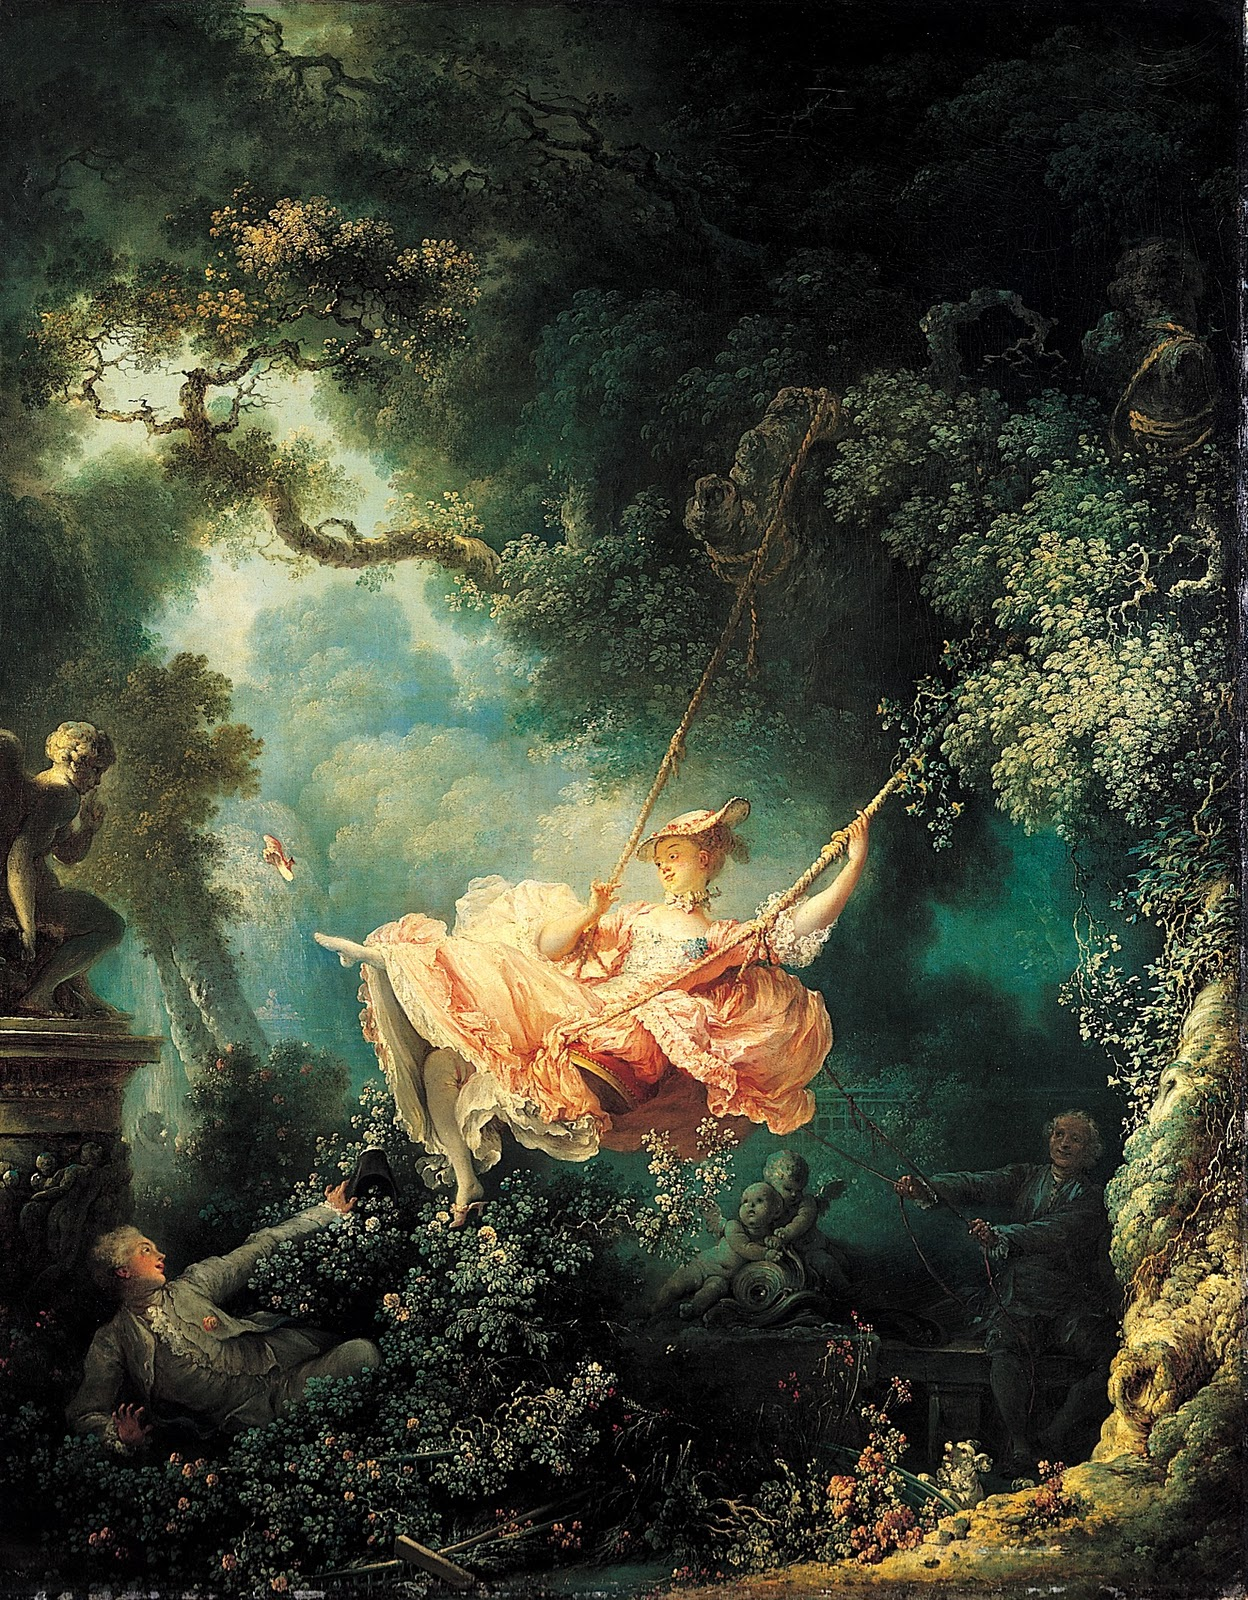
\includegraphics[scale=0.4, keepaspectratio=true]{qiuqian.jpg}
  \caption[让·奥诺雷·弗拉戈纳尔:《秋千》]{让·奥诺雷·弗拉戈纳尔:《秋千》。1767 年。布面油画。}\label{fig-qiuqian}

\end{figure}

